\documentclass[conference]{IEEEtran}

\usepackage[utf8]{inputenc}
\usepackage{cite}
\ifCLASSINFOpdf
  \usepackage[pdftex]{graphicx}
\else
  \usepackage[dvips]{graphicx}
\fi
\usepackage{amsmath}
\usepackage{array}
\usepackage{url}
\usepackage{paralist}
\usepackage{enumitem}
% correct bad hyphenation here
% \hyphenation{op-tical net-works semi-conduc-tor}

\begin{document}
% paper title
% Titles are generally capitalized except for words such as a, an, and, as,
% at, but, by, for, in, nor, of, on, or, the, to and up, which are usually
% not capitalized unless they are the first or last word of the title.
% Linebreaks \\ can be used within to get better formatting as desired.
% Do not put math or special symbols in the title.
\title{An Introduction to Clean Software Architecture}

\author{\IEEEauthorblockN{Péter Ivanics}
\IEEEauthorblockA{Department of Computer Science \\
University of Helsinki \\
Email: peter.ivanics@helsinki.fi \\
\url{http://pivanics.users.cs.helsinki.fi/portfolio/}}}

\maketitle

% As a general rule, do not put math, special symbols or citations
% in the abstract
\begin{abstract}
%<Context>
The construction and the long-term maintenance of robust software architecture is a demanding task. Software architects often face the problem to ensure the extensibility of systems so that new components can be added and existing ones can be removed or replaced easily. Linearly with software growth, these aspects of software engineering are getting more and more difficult because often times the separation of concerns and the decoupling of components are not considered in the beginning of the development.

%<Objectives>
The concept of the Clean Software Architecture was introduced recently by professional craftsmen in order to provide principles on how to achieve long-term robustness in software architecture engineering. This approach builds on top of the clean separation of concerns, finding the right abstractions on every level of the software projects, the minimal number of internal dependencies and finding the right flow of control.

%<Methods and objectives>
The objective of this study is to review relevant professional literature and summarize the most important aspects of the Clean Software Architecture. The paper describes the benefits of this approach compared to other practices. It is explained how this approach facilitates and why is it well-suited for Object Oriented principles and software projects of the present time. 

%<Results>
Results show that understanding the key concepts, such as The Dependency Rule and the core four layers of the Clean Architecture help developers to maintain robustness in their software. Ultimately, the concepts explained by this approach are independent from technologies and therefore easy to apply in many fields of our industry. 
\end{abstract}

\begin{IEEEkeywords}
Software architecture, Clean Code, Software development, Refactoring, Technical dept
\end{IEEEkeywords}

\section{Introduction}
% what is the context?
The construction and the maintenance of software is a difficult task from many aspects. Software development is a creative act of action where developers build intangible means from nothing \cite{cleancoder}. Linearly with the growth of the code base of a software project, its complexity and cost of change increases \cite{codecomplete} \cite{cleancode}, which makes developers' job even more difficult. 

% why talking about this is important? 
Software assets can be crucial for operations in industrial, business and research fields \cite{cleancode} \cite{cleancoder}. In the present time, more and more companies are established around providing software services to their customers \cite{cusumano2008changing}, and therefore software components can become business-critical. For this reason, the process of software development requires dedicated professionals with a lot of discipline, humility, dedication and commitment to their job \cite{cleancode}. 

% what can be the result of not paying attention to this and what are the ways to go?
Despite all the previously established standards and practices, developers often face troubles of conforming to the standards and understanding code written by others or even themselves \cite{cleancoder}. Keeping the code base maintainable, easy to understand and open for extensions is often a challenging task \cite{cleancoder}, but yet essential aspect to avoid paying the technical dept. For this reason, the concept of Clean Code \cite{cleancode} was established which further raised the attention towards maintainable software in the industry. Similarly, agile methods and principles became popular in order to facilitate developer productivity. 

% what is CC and what does it provide?
Clean Code is a concept introduced by Robert C. Martin \cite{cleancode} \cite{cleancoder}. This approach to software development aims for the delivery of elegant, easy to read, fully tested code base, in order to create robust, bug-free applications \cite{cleancode}. Additionally, the regular need for refactoring is emphasied as increases quality of software \cite{impactofrefactoring}, and therefore developers should not be afraid of performing this activity \cite{cleancoder}. 

% why and where is CC popular?
The Clean Code principles are getting more and more popular among wide range of software developers in the industry. On top of that, even universities consider to change their approach how to teach software development by introducing testing and maintainable code first to the students \cite{studentscleancode}. The reasons for its popularity are understandable: the principles are simple and clearly expressed, everyone who ever dealt with software development can relate to them and utilize the acquired knowledge right away. 

% how does this relate to softare architecture?
Software architectures lay down the basis and establish the frame for quality software. During the last decades, many different approaches and design patterns were developed and proposed by professionals to facilitate robustness of programs through design patterns \cite{codecomplete} \cite{onionarchitecture} \cite{gof}, which are widely used and appreciated by others worldwide. In order to ensure maintainable and robust software systems a loosely coupled, flexible and extensible frame should be provided as the basis, which is ready to accept continuously changing and new requirements. For this reason, an approach towards the Clean Software Architecture is emerging \cite{cleanarchitecture} building on top of Clean Code principles. 

% research questions of this paper
This paper aims to seek answers to the following research questions by discussing relevant literature in the topic: 

\setdefaultleftmargin{40pt}{}{}{}{}{}
\begin{enumerate}[label=RQ\arabic*:]
	\item what are the main aspects of the Clean principles in terms of software architecture?
	\item why such architecture is needed?
	\item how can any software project - independently from utilized technologies and platforms - benefit from the Clean Architecture principles?
\end{enumerate}  

% how is the rest of the paper structured? 
The rest of this paper is structured, as follows. The next section explains why a clean design for software architecture is needed and who may benefit approaching software development from this scope. Section III lists and discusses the four main principles and benefits of using a Clean Architecture for any software project. Finally, the last section concludes the findings of this research and establishes the directions for further studies in the topic. 

\section{The need for a clean design}
% why is software development and extending the code base difficult?
Software development is collaborative work. More and more developers work in teams of various sizes on multiple technologies to develop their software day-by-day. Inevitably, components are developed simultaneously by multiple coders and are getting bigger by time. As time passes, developers tend to have difficulties understanding the code they have written, because they do not remember what the intention behind the lines were \cite{cleancoder}. Similarly, understanding decisions made and code written by fellow colleagues is even more difficult and challenging on every level of abstraction \cite{cleancoder}. As the code base grows, decisions that were previously made may need to be reconsidered and code may need to be refactored to enhance its reliability and to avoid technical dept. 

% how can intent-driven approach help to get over this?
For this reason, considering the intent behind a decision is key even on the deepest level of components, for instance classes, objects, functions or even variable names. The usage of intention-revealing names on all parts of software projects greatly enhance the readability of their code \cite{cleancode}. This enables developers to read and understand others' code more efficiently and work on code written by others with more confidence. 

Demonstrating the intent behind design decisions is a key characteristic of good design which helps developers to understand what the program code does and how it is structured. This is particularly important while debugging or refactoring detailed parts of the code. However, it is not limited to low-level components of the software. 

% why is it important to understand the intents on every level of abstracition? 
Naturally, a complex system is composed of multiple components on different levels. In order to understand the "big picture" of such system, one may want to look at it on the top level from different angles. If an "outsider" (i.e. a new developer or system architect to the software) looks at a complex system, they may find it inconvenient, hard to understand or confusing at first, if the components, connection points or relationships are not named properly. 

As soon as components hold the property of telling their role at once in the ecosystem, it becomes much easier to understand. Clean naming conventions, for all components and their relationship strongly enhance the understandability of the system for individuals \cite{cleancode}. On top of that, intent-revealing components typically easy to adapt to the other key principles of clean design that are explained in the following section.

\section{Principles}
% what is the next step after demonstrating intent?
Communicating the intent behind the components is a good start for a Clean Software Architecture. Nevertheless, there are some other principles which help developers to avoid tight coupling and complex connections between the entities. The aim should be an approach, where each component is standalone and is handled as plugin to other parts of the application \cite{cleancode} \cite{cleanarchitecture}. In other words, components should be independent, which leads to the first principle of Clean Architecture, namely, the onion-like separation of architectural layers \cite{cleanarchitecture}. 

\subsection{Architectural Layers}
% what is a typical problem of system architecture? 
Many of the commonly used system-level design patterns may be easy to understand and implement, but are also hard to scale up to bigger systems. For example, the traditional Model-View-Controller (MVC) approach defines three main layers, namely user interface, business logic and database for the software. MVC is widely used in the industry due to its simplicity, however it carries the risk of tight coupling between the layers of the architecture as well as the difficult separation of concerns \cite{onionarchitecture}. 

% why MVC and similar patterns are not necesseraly scaleable? 
Tight coupling of the layers immediately leads to a hardly-scalable architecture unless the software is relatively small \cite{onionarchitecture}. As time passes, components grow bigger, at the same time technology develops and requirements change. Tightly coupled systems have hard time to follow-up on such changes, which is inevitable in case of business-critical systems \cite{onionarchitecture}. Therefore, a flexible and scalable approach to architectural layers is needed, which is flexible enough to support rapid system growth. 

% what is the solution? what does the onion architecture?
The solution to achieve a flexible, largely scalable architecture lies within the definition of the correct layers and the simple dependencies between them \cite{cleanarchitecture} \cite{onionarchitecture}. For instance, the Onion Architecture \cite{onionarchitecture} suggests to define the layers from inside-out, from core entities to to infrastructure as shown on Fig. \ref{cleanachitecture_fig}. 

\begin{figure}[!t]
\centering
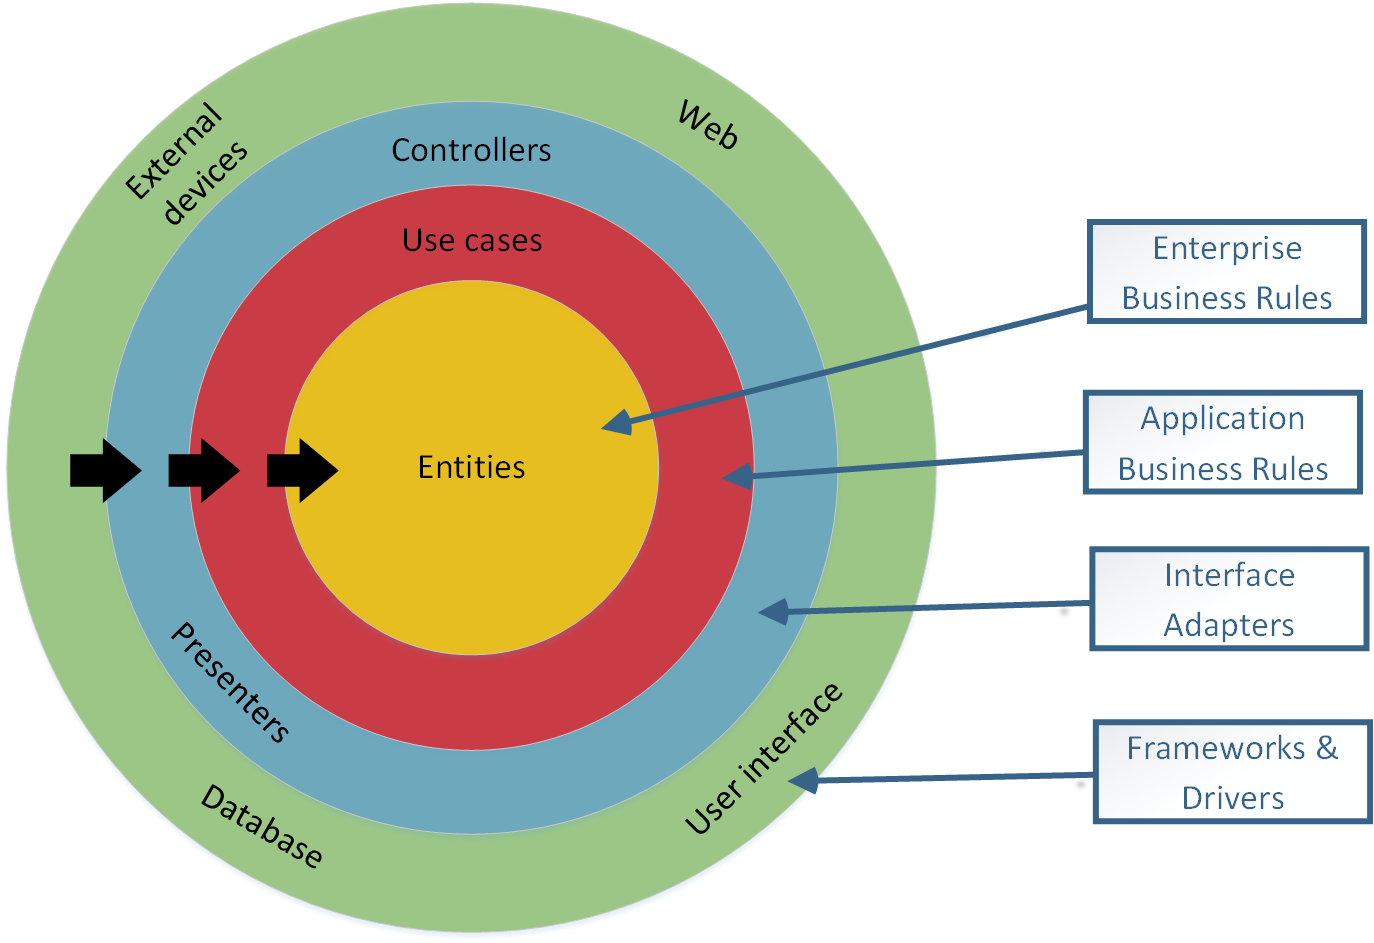
\includegraphics[width=3in]{images/cleanarchitecture.png}
\caption{The layers of the Clean Architecture and their inward-pointing dependencies (adapted from \cite{cleanarchitecture}).}
\label{cleanachitecture_fig}
\end{figure}

% what does the Onion Architecture suggest? 
The centermost layer, the Enterprise Business Rules define the domain specific business-entities and the domain-specific business logic. The responsibility of this layer is strictly limited to define entities and specific logic that are specific for the application's domain. More general functionality, that can be reused in other applications is delegated to the layers further away from the center. The Application Business Rules layer around the models is responsible to implement the business logic upon the business objects. As R. C. Martin points out \cite{cleanarchitecture}: \textit{"The outer circles are mechanisms. The inner circles are policies"}. 

Interface Adapters act as facilitators between the business logic and the events happening in the user interface, external input sources and the database \cite{onionarchitecture} \cite{cleanarchitecture}. This means that the business logic is defined closely on top of the entities and the external components, such as user interface or database control the entities through the rules indirectly. This greatly helps developers to distinguish the level of abstraction for every layer. 

% why is this good? 
Decoupling of different roles and the separation of responsibilities are key aspects in this design. Every layer has one task to cover and each holds the property of being possible to remove and replace by another component that has similar behavior but different internal logic. This kind of isolation embraces layers to be plugins to eachother and therefore easy to modify, extend or even replace during future development.

The four layers shown on Fig. \ref{cleanachitecture_fig} create the core of a Clean Architecture. Nevertheless, as systems grow bigger, they may divide layers and separate them even further. For example, one may divide entity model objects from their business logic to have an even more clear distinction of roles among the components.

\subsection{Separation of concerns}
A well-designed system-wide architecture also aims to separate concerns. By separating responsibilities in the application well, the code not only gets easier to understand but also more flexible, loosely coupled and easier to test  \cite{cleancoder} \cite{cleanarchitecture} \cite{onionarchitecture}. This helps to tell the responsibility and place the components by their names to the correct layers described in the previous section.

Consequently, to allow understanding the software architecture on its highest level, clear decisions should be made on the responsibility of the components. Once the components are chosen, their name should tell right away the intent they were made for. Applying the same approach on every level of abstraction throughout the application is crucial as it keeps components minimal, and lightweight. 

\subsection{The Dependency Rule}
The approach to a layered architecture also requires the definition of carefully designed dependencies. Identifying the correct dependencies and keeping them minimal is key to a loosely coupled software \cite{cleancode}. The Clean Architecture explained in the previous sections is designed in a way, that such dependencies are considered at the first place.

% what does the dependency rule say?
The Dependency Rules dictates that the inner layers of the architecture do not know anything about the layers that are outer than them in the architecture \cite{cleanarchitecture} \cite{onionarchitecture}. In other words, all dependencies point towards the middle of the layered structure, towards the business logic and the entities. 

% how does this help in the long run?
Consequently, individual layers do not know about in which context they are being used, but they know the insides of the encapsulated entities underneath their level. The deeper we go into the architecture, the less dependencies exist and less complications are experienced. 

This approach allows the layers to be plugins to eachother: in case one of the mechanisms (for instance the user interface or database) change, it is sufficient to replace its layer and conform it to the interfaces \cite{cleanarchitecture} \cite{onionarchitecture}. As soon as correct interfaces are defined the edges of the layers, such mechanisms become immediately external. This kind of decoupling greatly lowers the maintenance cost for the lifetime of an application \cite{onionarchitecture}. On top of that, the software becomes more flexible and adapts to new or changing requirements easier. 

\subsection{Flow of control}
% how is the two-way communication handled? 
Crossing the boundaries from inside out may be required in certain situations. For example, if an action initiated by a Controller object has an impact on the business logic and thus on the state of the entities, the user interface or the database may need to be updated once the changes are committed. For this reason, the layers should be designed in a manner that they take inputs on one interface and produce output on another \cite{cleanarchitecture}. The mechanism which is to handle the output can respond to the received data and perform the necessary actions accordingly. 

\begin{figure}[!t]
\centering
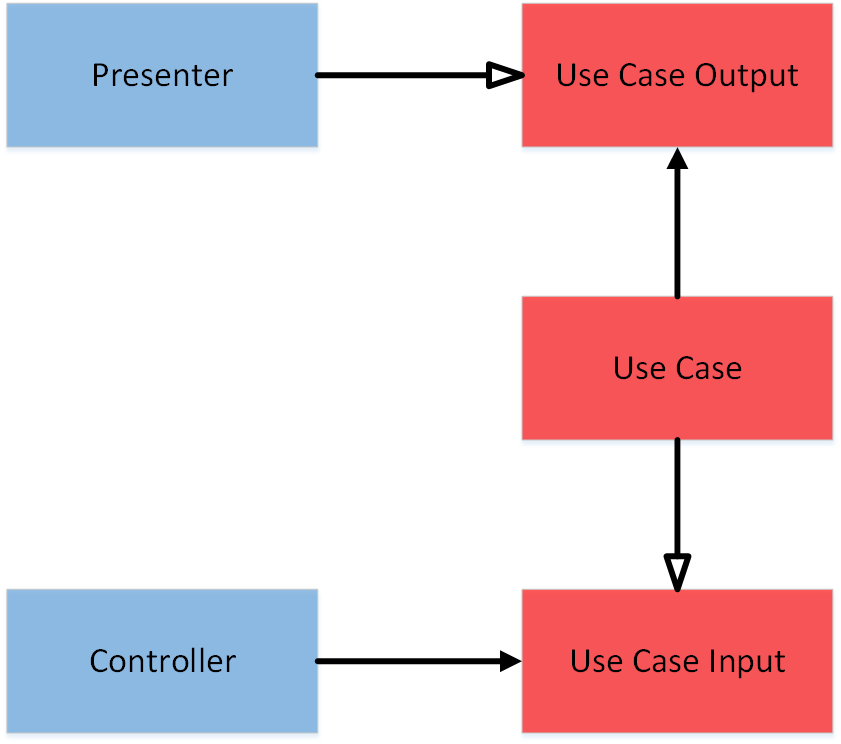
\includegraphics[width=2.5in]{images/flowcontrol.png}
\caption{The flow of control between neighbouring layers in the Clean Architecture \cite{cleanarchitecture}. The filled arrows represent data submission to, the hollow arrows data retrieval from the pointed component.}
\label{flowcontrol}
\end{figure}

% explain the figure flowcontrol
As shown on Fig. \ref{flowcontrol}, the control flow goes through interfaces when the boundaries are crossed. The layer which is closer towards the center of the architecture receives data through its input interface, processes it and passes it forward on its output interface. More specifically, a Controller object may trigger an event to process some data in a Use Case, which data is then forwarded through the output interface and presented in the necessary component. 

This way each layer encapsulates its own logic. The responsibilities remain clearly separated and the Dependecy Rule is not violated, because layers do not know anything of the insides of the others. The inner layer passes data back to an outer layer through an interface, that is implemented in the receiver class. This is called the Dependency Inversion Principle \cite{cleanarchitecture} \cite{onionarchitecture}. 

% what data crosses the boundaries?
For simplicity, it is suggested that the interfaces deal with simple data types \cite{cleanarchitecture}. For the sake of not violating the Dependency Rule, the inner circles should expose their objects and data structures when passing data to an interface. Therefore, it is suggested to define the interfaces such that only simple data structures cross the boundaries \cite{cleanarchitecture}. 

\subsection{Testability}
The layered structure and inward-pointing dependencies have other benefits than flexibility and easy maintenance. Due to the fact that every layer has interfaces (some may call them input and output ports), they become easy to test \cite{cleanarchitecture}. 

Automated testing is another great tool which can contribute to the robustness of the software, because it allows developers to have confidence in their software \cite{cleancoder}. Running automated tests does not take too much effort or time as soon as they are written. It does not matter if existing components of the project have to be refactored, replaced or new functions are to be added, automation can always increase productivity and quality assurance in this context \cite{cleancode}. 

Making continuous changes to the software is inevitable, because software components extend, hence change and are refactored every now and then. Once automated tests are set up, developers will have confidence to change confusion, inefficient or tightly coupled parts of the application \cite{cleancoder}. Seeing the test coverage data and the green stage of automated tests gives the confidence of quality in their code base. As R.C. Martin points out, software developers  \textit{"are afraid they will break it (their code) (...) Because they do not have tests."} \cite{cleancoder}

Consequently, testing the layered architecture is possible and strongly suggested on every level of detail. This property greatly contributes to continuous development, developer productivity and quality assurance. On top of that, technical dept becomes easier to manage and avoid. 

%\subsection{Platform independence}
%Due to its abstract structure, this approach to software architecture is not only robust and flexible, but also independent from platform and the the utilized tools. 

\section{Conclusion}
% restate the topic
The construction and the maintenance of software is a demanding and difficult task. As time passes, many components grow too big or get outdated, which asks for the refactoring of the code base. In many cases, the underlying software architecture is coupled too tightly, which makes developers' job difficult to extend their software. Therefore, software architecture forms the frame of every software application.

% summarize main points
Accordingly, there is need for a good, robust and flexible design to ensure the avoidance of technical dept and keep the code base robust as well as extensible. Many design patterns on multiple level of abstractions were suggested by researchers in the past to help developers achieve such goals. Recently, the principles of Clean Code were introduced in the industry, based on which the Clean Software Architecture is emerging. 

The Clean Code suggests an intent-driven approach to software development. This means all code that is written, should clearly communicate the reason why it was written and explicitly tell what it is doing. The Clean Software Architecture adapts this rule and puts it in relationship with software architecture, where the components are expected to be placed, connected and named with intention. 

Additionally, this approach to software architecture embraces principles, such as the separation of concerns, the dependency rule and the inward-pointing flow of control. As soon as these criterion is matched, faster deployment, more robust and flexible software architecture is guaranteed. 

This paper introduced the above concepts in relation to software development based review of relevant literature. It was concluded that the Clean principles can be adapted to software architecture design, which help developers to collaborate, ensure quality software and to avoid technical dept in the long run. Another finding concerning this approach to development is the decoupled and testable components it provides, which are theoretically independent from platform and easy to replace. 

It was shown what the most important approaches towards a Clean Software Architecture are and how it can be achieved. Some of the most important advantages were pointed out and summarized in this paper. Further research in this topic may involve a case study or practical analysis on the topic. 

\begin{thebibliography}{1}

  \bibitem{cleanarchitecture}
R. C. Martin. (2012, Aug. 13) \emph{The Clean Architecture} [Online]. Available: \url{https://8thlight.com/blog/uncle-bob/2012/08/13/the-clean-architecture.html}

\bibitem{cleancoder}
R. C. Martin. \emph{The Clean Coder: A Code of Conduct for Professional Programmers}, 1st ed. Boston, MA, Pearson Education, Inc. 2011. 

\bibitem{cleancode}
R. C. Martin. \emph{Clean Code: A Handbook of Agile Software Craftsmanship}, 1st ed. Boston, MA, Pearson Education, Inc. 2008.

\bibitem{onionarchitecture}
J. Palermo. \emph{The Onion Architecture} [Online]. Available: \url{http://jeffreypalermo.com/blog/the-onion-architecture-part-1/}

\bibitem{codecomplete}
S. Steve McConnell. \emph{Code Complete: A Practical Handbook of Software Construction}, 2nd ed. Microsoft Press. 2004.

\bibitem{cusumano2008changing}
M. Cusumano. \emph{The Changing Software Business: From Products to Services and Other New Business Models Paper 236}. MIT Center for Digital Business. 2007.

\bibitem{gof}
E. Gamma, R. Helm, R. Johnson, J. Vlissides \emph{Design Patterns: Elements of Reusable Object-Oriented Software}, 1st ed. Addison Wesley. 1994.

\bibitem{impactofrefactoring}
M. Wahler, U. Drofenik, W. Snipes. \emph{Improving Code Maintainability: A Case Study on the Impact of Refactoring}. 2016 IEEE International Conference on Software Maintenance and Evolution. 2016.

\bibitem{studentscleancode}
M. Doyle, B. Buckley, W. Hao,  J. Walden. \emph{Work in Progress - Does Maintenance First Improve Student's Understanding and Appreciation of Clean Code and Documentation}. Frontiers in Education Conference (FIE). 2011.
% http://hillside.net/patterns

% Swift Design Patterns: The Easy Way; Standard Solutions for Everyday Programming Problems; Great for: Game Programming, System Analysis, App Programming, ... & Database Systems (Design Patterns Series) https://www.amazon.com/Swift-Design-Patterns-Solutions-Programming-ebook/dp/B01N2KE1T7/ref=sr_1_8?ie=UTF8&qid=1488874232&sr=8-8&keywords=software+patterns

\end{thebibliography}
\end{document}
